\chapter{Bash脚本}
\label{sec:shellScript}
\index{bash}

无聊地重复一件事确实惹人厌!当然了,数次重复一些命令是不是也是很不爽的
一件事呢?如果是请跟随我往下看。当我们熟悉了操作系统后,以期望有更好的
提高,那就是写脚本了。

\section{正则表达式}

Regular expression\index{Regular Expression} (abbreviated regex or
regexp) is a sequence of characters that forms a search pattern,
mainly for use in pattern matching with strings, or string matching,
i.e. "find and replace"\-like operations.

正则表达式就是由一系列特殊字符组成的字符串, 其中每个特殊字符都被称为元
字符, 这些元字符并不表示为它们字面上的含义, 而会被解释为一些特定的含义.
具个例子, 比如引用符号, 可能就是表示某人的演讲内容, 同上, 也可能表示为
我们下面将要讲到的符号的元-含义. 正则表达式其实是由普通字符和元字符共同
组成的集合, 这个集合用来匹配(或指定)模式.

一个正则表达式会包含下列一项或多项:

\begin{enumerate}[itemsep=0pt,parsep=0pt]
\item 一个字符集. 这里所指的字符集只包含普通字符, 这些字符只表示它们的
  字面含义. 正则表达式的最简单形式就是只包含字符集, 而不包含元字符.
\item 锚. 锚指定了正则表达式所要匹配的文本在文本行中所处的位置. 比如,
  \^, 和\$就是锚.
\item 修饰符. 它们扩大或缩小(修改)了正则表达式匹配文本的范围. 修饰符包
  含星号, 括号, 和反斜杠.
\end{enumerate}

\subsection{正则表达式语法}

\subsection{一些实例}


\section{awk}
\label{sec:awk}

如果要格式化报文或从一个大的文本文件中抽取数据包,那么awk可以完成这些任
务。它在文本浏览和数据的熟练使用上性能优异。与其它大多数Unix/Linux命令
不同的是,从名字上看,我们一眼看不出awk\index{awk}的功能:它既不是具有独立意义的英
文单词,也不是几个相关单词的缩写。事实上,awk是三个人名的缩写,他们是:
Aho、(Peter) Weinberg和(Brain)Kernighan。正是这三个家伙创造了awk,一个
优秀的样式扫描与处理工具。本章只介绍Gnu的awk版本gawk,其他awk版本不做介
绍。

awk的工作流程:
\begin{figure}[!htbp]
  \centering
  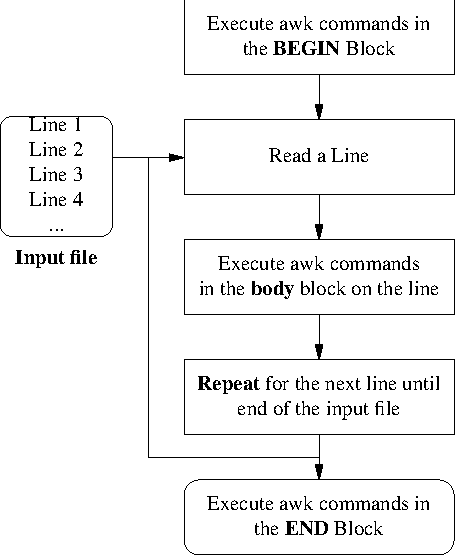
\includegraphics[width=.5\textwidth]{graph/awk_workflow.pdf}
  \caption{awk工作流程}
  \label{fig:awk_workflow}
\end{figure}

\subsection{初步使用}
\label{subsec:FirstAwk}

假如我们有文件employee.txt,内容如下:

\begin{verbatim}
Beth	4.00	0
Dan	3.75	0
Kathy	4.00	10
Mark	5.00	20
Mary	6.50	22
Susie	6.25	18
\end{verbatim}

第一列表示员工姓名,第二列表示每小时加班所得的人民币,第三列为加班多少
小时。我们现在就来打印出那些加班大于0个小时的员工及其加班费,在命令行只
需执行这样一行命令即可:

\begin{verbatim}
# awk '$3 > 0 { print $1, $2 * $3 }' employee.txt
\end{verbatim}

我们会得到这样的输出:

\begin{verbatim}
Kathy 40
Mark 100
Mary 143
Susie 112.5
\end{verbatim}

上面的命令告诉系统运行awk,使用单引号里的程序,并从employee.txt文件里获
得自己的数据。单引号里的部分完全就是awk程序。它包含了单个的
pattern-action(模式-动作)语句。动作\$3 >  0,匹配输入的每一行的第三列
或域,如果该列大于0,然后就执行下面的动作

\begin{verbatim}
{ print $1, $2 * $3 }
\end{verbatim}

对于每匹配到的行,就会打印第一个域并同时计算第二个域与第三个域的乘积。

如果我们想看看哪个家伙这个月没有加班,可以使用下面的命令:

\begin{verbatim}
# awk '$3 == 0 { print $1 }' employee.txt
\end{verbatim}

这里的模式,\$3 == 0,将会匹配每一输入行的第三个域,如果等于0,就会执行
下面的动作

\begin{verbatim}
{ print $1 }
\end{verbatim}

打印第一个域。

\subsection{awk程序结构}

awk的基本操作是对输入的行做逐一扫描,搜索这些行中匹配到的任意模式,然后
执行相应的动作。然后下一行被读进来并从头开始匹配到行末,直到输入文件的
所有行被读进来。就\$3 > 0来说,当满足时,说明该条件为真。

在上面的例子中,只有一个模式和动作,可以称为单pattern-action语句;对于
每一行,匹配到第三个字段等于0时,第一个字段将会被打印。

另外,模式和动作并不总是成对出现的,就是说,在pattern-action语句中,可
能只有模式或者只有动作。如果一个pattern没有相应的action,例如,

\begin{verbatim}
$3 == 0
\end{verbatim}

然后,每一被匹配的行都将会被打印,

\begin{verbatim}
Beth    4.00    0
Dan     3.75    0
\end{verbatim}

如果一个action没有pattern时,例如,

\begin{verbatim}
{ print $1 }
\end{verbatim}

此时,将会打印每一行的第一个域。由上可知,patterns和actions都是可选的。
actions使用大括号括起来以与patterns区分。

\subsection{BEGIN与END}

特殊的BEGIN模式在第一个输入文件的第一行被匹配,而END则是在最后一个文件的最后被处理后匹配。
下面的程序将会打印一个头部:

\begin{verbatim}
BEGIN { print "NAME     RATE    HOURS"; print "" }
      { print }
\end{verbatim}

我们将会得到这样的输出:

\begin{verbatim}
NAME     RATE   HOURS

Beth     4.00   0
Dan      3.75   0
Kathy    4.00   10
Mark     5.00   20
Mary     6.50   22
Susie    6.25   18
\end{verbatim}

我们可以在一行同时输入多条语句,这些语句之间需要用分号分开。注意
到,\textit{print ""}意思是打印一个空行,它与print不一样,仅仅一
个print语句将打印整行。

\subsection{域和记录}
\label{subsec:FieldRecordAwk}

awk执行时,其浏览域标记为\$1,\$2,...\$n。这种方法称为域标识。使用这些
域标识将更容易对域进一步处理。

\subsection{内置变量}

awk有一些内置的变量,变量如下:

\begin{table}[hbtp]
  \begin{center}
    \begin{tabular}{ll}
      \hline
      变量     & 说明 \\
      \hline
      ARGC        & 命令行中参数的个数 \\
      \hline
      ARGV        & 包含命令行参数的数组 \\
      \hline
      CONVFMT     & 用于数字的字符串转换格式(默认格式为\%.6g) \\
      \hline
      ENVIRON     & 环境变量的关联数组 \\
      \hline
      FILENAME    & 当前文件名 \\
      \hline
      NR          & 当前记录的个数(当前的行号) \\
      \hline
      FNR         &  当前记录的个数(仅为当前文件,而非全部输入文件) \\
      \hline
      FS          & 字段分割符(默认为空格) \\
      \hline
      NF          & 当前记录中的字段个数 \\
      \hline 
      OFMT        & 数字的输出格式(默认格式为\%.6g) \\
      \hline
      OFS         & 输出字符的分割符(默认为空格) \\
      \hline
      ORS         & 输出记录分割符(默认为换行) \\
      \hline
    \end{tabular}
  \end{center}
\end{table}

\subsection{One-liners awk程序}

这一节介绍几个很有用的、短小精悍的awk程序。

\begin{enumerate}
\item 打印输入文件的总行数
\item 打印指定的行
\item 打印输入行的最后一个字段
\item 打印最后一行的最后一个字段
\item 打印每一输入行并擦除第二个字段
\end{enumerate}

\subsection{条件和循环}

这一节包含了一些基本的编程结构。它覆盖了awk程序设计语言中的所有控制结构。
在awk中,这些条件和循环的语法用起来比较简单。实际上,awk中的条件和循环
结构的语法借鉴C语言。因此,通过学习awk,我们也同样在学习C语言。

\subsection{if-else语句}

awk提供一个\textit{if-else}语句,这些语句只能用在actions中。下面的这个
程序使用的还是\ref{sec:FirstAwk}节的例子。在这个例子中,我们会计算那些
每小时加班费大于6块的家伙,他们的总加班费及平均加班费。

\begin{verbatim}
# cat progfile
$2 > 6 { n = n + 1; pay = pay + $2 * $3 }
END    { if (n > 0)
            print n, "employees, total pay is", pay,
                     "average pay is", pay / n
         else
            print "no employees are paid more than Y6/hour"
}

# awk -f progfile employee.txt
\end{verbatim}

我们将会得到下面的输出结果:

\begin{verbatim}
  2 employees, total pay is 255.5 average pay is 127.75
\end{verbatim}

\subsection{while循环}
\label{subsec:WhileLoop}

while语句有一个condition和一个body。当condition为真时,body中的语句将被重复执行。我们使用下面的
程序计算这样的一个公式$ value = amount(1+rate)^{years} $

\begin{verbatim}
  # cat interest1 
  # interest1 - compute compound interest
  #   formula: value = amount(1+rate)^years
  #   input: amount rate years
  #   output: compounded value at the end of each year
  
  {  i = 1
    while (i <= $3) {
      printf("\t%.2f\n", $1 * (1 + $2) ^ i)
      i = i + 1
    }
  }
\end{verbatim}

如何执行该程序?看操作,

\begin{verbatim}
  # awk -f interest1 <- 回车
  1000 .06 5 <- 输入三组数字后,回车
  1060.00
  1123.60
  1191.02
  1262.48
  1338.23
\end{verbatim}

\subsection{for循环}
\label{subsec:ForLoop}

我们使用for语句改写第\ref{subsec:WhileLoop}节的while程序。如下:

\begin{verbatim}
  # cat interest2
  # interest2 - compute compound interest
  #   formula: value = amount(1+rate)^years
  #   input: amount rate years
  #   output: compounded value at the end of each year
  
  {  for (i = 1; i <= $3; i = i + 1)
    printf("\t%.2f\n", $1 * (1 + $2) ^ i)
  }
\end{verbatim}

\subsection{do循环}

\subsection{影响流控制的语句}

\subsection{数组}

数组是可以用来存储一组数据的变量。通常这些数据之间具有某种关系。数组中
的每一个元素通过它们在数组中的下标来访问。每个下标用方括号括起来。下面
的语句表示为数组中的一个元素赋值。

\begin{verbatim}
  array[subscript] = value
\end{verbatim}

在awk中不必指明数组的大小,只需要为数组指定标示符。向数组元素赋值比较容
易。例如,下面的例子中为数组hr的一个元素指定了一个字符串“laven”。

\begin{verbatim}
  hr[1] = "laven"
\end{verbatim}

这个数组元素的下标是“1”,下面的语句将打印字符串“laven”。

\begin{verbatim}
  print hr[1]
\end{verbatim}

当然,我们可以用循环向数组中写入或取出元素。例如,如果数组hr有10个元素,
可以使用下面的循环来打印每个元素:

\begin{verbatim}
  hr_count = 10
  for (x = 1; x <= hr_count; ++x)
  print hr[x]
\end{verbatim}

我们来看一个例子,依然使用第\ref{sec:FirstAwk}节中的输入文件,让employee.txt文件反序输出,

\begin{verbatim}
# cat reverse
# reverse - print input in reverse order by line
{ line[NR] = $0 } # remember each input line
END  { i = NR          # print lines in reverse order
  while (i > 0) {
    print line[i]
    i = i - 1
  }
}
  
# awk -f reverse employee.txt
Susie    6.25   18
Mary     6.50   22
Mark     5.00   20
Kathy    4.00   10
Dan      3.75   0
Beth     4.00   0
\end{verbatim}

\subsection{表达式}

\begin{verbatim}
# cat awk_file 
gold     1    1986  USA                 American Eagle
gold     1    1908  Austria-Hungary     Franz Josef 100 Korona
silver  10    1981  USA                 ingot
gold     1    1984  Switzerland         ingot
gold     1    1979  RSA                 Krugerrand
gold     0.5  1981  RSA                 Krugerrand
gold     0.1  1986  PRC                 Panda
silver   1    1986  USA                 Liberty dollar
gold     0.25 1986  USA                 Liberty 5-dollar piece
silver   0.5  1986  USA                 Liberty 50-cent piece
silver   1    1987  USA                 Constitution dollar
gold     0.25 1987  USA                 Constitution 5-dollar piece
gold     1    1988  Canada              Maple Leaf
\end{verbatim}

\begin{verbatim}
# This is an awk program that summarizes a coin collection.
#
/gold/    { num_gold++; wt_gold += $2 }    # Get weight of gold.
/silver/  { num_silver++; wt_silver += $2 }# Get weight of silver.
END { val_gold = 485 * wt_gold;            # Compute value of gold.
    val_silver = 16 * wt_silver;         # Compute value of silver.
    total = val_gold + val_silver;
    print "Summary data for coin collection:";  # Print results.
    printf ("\n");
    printf ("   Gold pieces:                 %2d\n", num_gold);
    printf ("   Weight of gold pieces:       %5.2f\n", wt_gold);
    printf ("   Value of gold pieces:        %7.2f\n",val_gold);
    printf ("\n");
    printf ("   Silver pieces:               %2d\n", num_silver);
    printf ("   Weight of silver pieces:     %5.2f\n", wt_silver);
    printf ("   Value of silver pieces:      %7.2f\n",val_silver);
    printf ("\n");
    printf ("   Total number of pieces:      %2d\n", NR);
    printf ("   Value of collection:         %7.2f\n", total);
}
\end{verbatim}

\begin{verbatim}
[root@unionpay bash]# awk -f myawk awk_file 
Summary data for coin collection:

   Gold pieces:                    9
   Weight of gold pieces:          6.10
   Value of gold pieces:        2958.50

   Silver pieces:                  4
   Weight of silver pieces:       12.50
   Value of silver pieces:       200.00

   Total number of pieces:        13
   Value of collection:         3158.50
\end{verbatim}

\subsection{函数}

\subsection{总结}


\section{sed}
\label{sec:sed}

Sed\index{sed}是一个超级流式编辑器。
picture a stream flowing through a pipe. Okay, you can't see a stream
if it's inside a pipe. That's what I get for attempting a flowing
analogy. You want literature, read James Joyce.

Anyhow, sed is a marvelous utility. Unfortunately, most people never
learn its real power. The language is very simple, but the
documentation is terrible. The Solaris on-line manual pages for sed
are five pages long, and two of those pages describe the 34 different
errors you can get. A program that spends as much space documenting
the errors than it does documenting the language has a serious
learning curve.

Do not fret! It is not your fault you don't understand sed. I will
cover sed completely. But I will describe the features in the order
that I learned them. I didn't learn everything at once. You don't need
to either.

sed的工作流程:
\begin{figure}[!htbp]
  \centering
  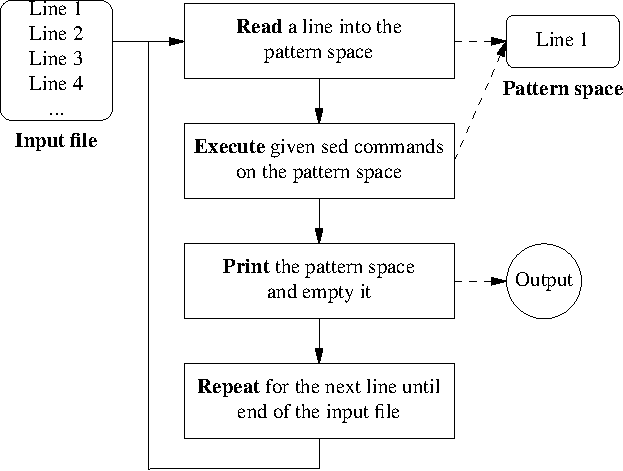
\includegraphics[width=.65\textwidth]{graph/sed_workflow.pdf}
    \caption{sed工作流程}
  \label{fig:sed_workflow}
\end{figure}

命令列表:

\begin{tabular}{lp{25em}}
\toprule
命令       & 说明 \\
\midrule
a          & 在当前行后面追加文本 \\
b label    & 分支到脚本中带有标号的地方,如果标号不存在就分支到脚本的末尾 \\
c          & 用新的文本改变或者替代本行的文本 \\
d          & 从模板块(Pattern space)位置删除行 \\
D          & 删除模板块的第一行 \\
i          & 在当前行上面插入文本 \\
h          & 拷贝模板块的内容到内存中的缓冲区 \\
H          & 追加模板块的内容到内存中的缓冲区 \\
g          & 获得内存缓冲区的内容,并替代当前模板块中的文本 \\
G          & 获得内存缓冲区的内容,并追加到当前模板块文本的后面 \\
l          & 列表不能打印字符的清单 \\
n          & 读取下一个输入行,用下一个命令处理新的行而不是用第一个命令 \\
N          & 追加下一个输入行到模板块后面并在二者之间嵌入一个新的行,改变当前行的号码 \\
p          & 打印模板块的行 \\
P          & 打印模板块的第一行 \\
q          & 退出 sed \\
r file     & 从file中读行 \\
t label    & if分支,从最后一行开始,条件一旦被满足或者T命令或者t命令, 将导致分支到带有标号的命令处,或者到脚本的末尾 \\
T label    & 错误分支,从最后一行开始,一旦发生错误或者T命令或者t命令, 将导致分支到带有标号的命令处,或者到脚本的末尾 \\
w file     & 写并追模板块到file末尾 \\
W file     & 写并追模板块的第一行到file末尾 \\
!          & 表示后面的命令对所有没有被选定的行发生作用 \\
s/re/string/ & 用string替换正则表达式re \\
=          & 打印当前行号码 \\
注释command & 把注释扩展到下一个换行符以前替换标记 \\
g           & 行内全面替换 \\
p           & 打印行 \\
w           & 把行写入一个文件 \\
x           & 互换模板块中的文本和缓冲区中的文本 \\
y           & 把一个字符翻译为另外的字符(但是不能用于正则表达式) \\
\bottomrule
\end{tabular}

一些选项:

\begin{tabular}{l|lp{20em}}
\hline
-e command             & 允许多点编辑 \\
\hline
--expression=command   & 同上 \\
\hline
-h,--help              & 打印命令行选项摘要,并显示 bug 列表的地址 \\
\hline
-n,--quiet,--silent    & 取消默认输出 \\
\hline
-f,                    & 引导 sed 脚本文件名 \\
\hline
--filr=script-file     & 同上 \\
\hline
-V,--version           & 打印版本和版权信息\\
\hline
\end{tabular}

\subsection{匹配}
\label{sec:sedPattern}

\subsection{变量定义}
\label{subsec:sedVariableDef}

\subsection{特殊变量}
\label{subsec:sedSpecialVariable}

\subsection{数组}
\label{subsec:sedArray}

\subsection{删除}
\label{subsec:sedDelete}

删除(d)编辑命令采用一个地址,如果行匹配这个地址就删除模式空间的内容。
删除命令(d)还是一个可以改变脚本中的控制流的命令。这是因为一旦执行这个
命令,那么在“空的”模式空间中就不会再有命令执行。删除命令(d)会导致读取
新输入行,而编辑脚本则从头开始新的一轮。重要的是,如果某行匹配这个地址,
那么就删除整个行,而不只是删除行中匹配的部分。

\subsection{替换}
 
Sed有众多命令,但经常被用到的就是最基本的替换命令“s”了, 替换命令有四部
分组成,如下表所示:

\begin{table}[h]
\centering
\begin{tabular}{l|l}
\hline
s	     & 所使用的命令是替换命令 \\
\hline
/../../	 & 所使用的分隔符,可以自行改变,不过三个符号要一致 \\
\hline
old	     & 这是将要被替换的字符串或正则表达式 \\
\hline
new	     & 这是替换后的字符串 \\
\hline
\end{tabular}
\end{table}

sed s/day/night/ <old >new

eg: sed 's/local/host/[g]' /etc/hosts
 
Or another way (for Unix beginners), 

sed s/day/night/ old >new
 
我们也可以如下这样写,

\small{
\begin{verbatim}
echo day | sed s/day/night/ 
\end{verbatim}
}
\normalsize

将会输出“night”。

我们在这里并没有使用引号把这些参数给引用起来,也能得出想要的结果,因为
这个例子是不需要它们的,嘿嘿!然而,在使用过程中出现了原字符,这时候引
号是必须要的。如果我们不确定何时要使用引号,那么,最好的习惯就是“每用
必带”引号即可,不用纠结那么多。

sed 's/day/night/' <old >new

I must emphasize that the sed editor changes exactly what you tell it
to. So if you executed
 
\begin{verbatim}
eg: # echo Sunday | sed 's/day/night/'
output: Sunnight
\end{verbatim}
 
This would output the word "Sunnight" bacause sed found the string
"day" in the input.
 
The search pattern is on the left hand side and the replacement string
is on the right hand side.
 
We've covered quoting and regular expressions. That's 90\% of the
effort needed to learn the substitute command. To put it another way,
you already know how to handle 90\% of the most frequent uses of
sed. There are a ... few fine points that an future sed expert should
know about. (You just finished section 1. There's only 63 more
sections to cover. :-) Oh. And you may want to bookmark this page,
.... just in case you don't finish.

\subsection{追加、插入和更改}
\label{subsec:appendInsertChange}

追加(a)、更改(c)、插入(i)编辑命令提供了类似于vi交互式编辑器的编辑功能。

追加命令(a)将文本放置在当前行之后。更改命令(c)用所指定的文本取代模
式空间的内容。插入命令(i)将所提供的文本放置在模式空间的当前行之前。这
些命令中的每一个都要求后面跟一个反斜杠用于转义第一个行尾。如要输入多行
文本,每个连续的行都必须用反斜杠结束,最后一行除外。而且,如果文本包含
一个字面含义的反斜杠,要再添加一个反斜杠来转义它。

\subsection{模式空间和保留空间}
\label{subsec:patternSpace}

\subsection{流控制}
\label{subsec:flowControl}

\subsection{地址范围}
\label{subsec:addrSpace}

\subsection{调用外部变量}
\label{subsec:callExternalVariable}

\subsection{总结}
\label{subsec:summary}



\section{语法介绍}

\subsection{变量定义}

\subsection{特殊变量}

在脚本里有以下几个特殊的变量,如下

\begin{table}[htbp]
  \centering
  \caption{特殊变量的含义}
  \label{tab:specialVariables}
  \begin{tabular}{cl}
    \toprule
    变量  & 说明 \\
    \midrule
    \$0   & 代表该脚本的名字 \\
    \$n   & 代表该程序的第n\footnote{如果参数超过10个,则使用\$n就不合适了,需要使用\$\{n\}的形式。}个参数值,n=1..9 \\
    \$*   & 代表该脚本的所有参数 \\
    \$\#  & 代表该脚本的参数个数 \\
    \$\$  & 代表该脚本的PID \\
    \$!   & 代表上一个指令的PID \\
    \$?   & 代表上一个指令的返回值 \\
    \bottomrule
  \end{tabular}
\end{table}

\subsection{变量赋值和替换}

\subsection{本地变量与全局变量}

\subsection{引用变量}

\subsection{数组}

Bash只支持一维数组,但参数个数没有限制。

数组赋值:

\begin{verbatim}
1. array=(var1 var2 var3 ... varN)
2. array=([0]=var1 [1]=var2 [2]=var3 ... [n]=varN)
3. array[0]=var1
   array[1]=var2
   array[2]=var3
   ...
   array[N]=varN
\end{verbatim}

\begin{verbatim}
  declare -

  MYARRAY=([0]=tom [1]=laven [2]=liu [5]=jim)
  
  数组的元素的长度:
  ${#MYARRAY} 指的是数组MYARRAY的第0个元素的长度,与
  ${#MYARRAY[0]} 等价
  ${#MYARRAY[n]} 是第n+1个元素,

  数组的元素个数:
  ${#MYARRAY[*]}
  ${#MYARRAY[@]}
\end{verbatim}
  一个例子,随机生成10个整型元素的的数组,并找出该数组中的最大值。
  \begin{lstlisting}
  #!/bin/bash
  #
  for i in {0..9}
  do
  ARRAY[$i]=$RANDOM
  echo -n "${ARRAY[$i]} "
  sleep 1
  done

  echo

  declare -i MAX=${ARRAY[0]}
  INDEX=$[${#ARRAY[*]-1}]
  for i in `seq 1 $INDEX`
  do
      if [ $MAX -lt ${ARRAY[$i]} ] ; then
          MAX=${ARRAY[$i]}
      fi
  done

  echo ${MAX}
  \end{lstlisting}

\subsection{特殊字符}

\section{基本流程}

Bash与其他编程语言一样,也有自己的程序处理逻辑。接下来的这个章节主要介
绍Bash的脚本几种基本流程。

\subsection{if结构}

先看一下bash的man page是如何定义if结构的,

\begin{figure}[!htbp]
  \centering
  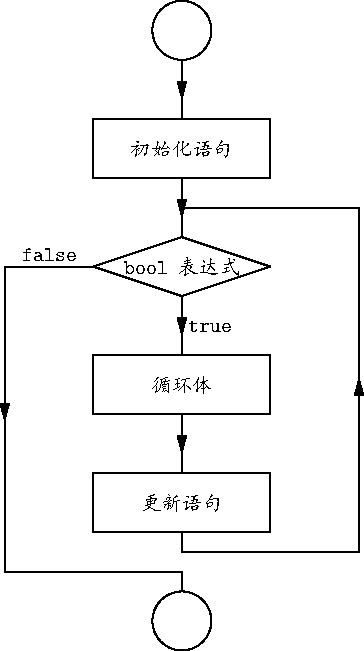
\includegraphics{graph/for.pdf}
    \caption{for工作流程}
  \label{fig:for_workflow}
\end{figure}

\begin{verbatim}
if list; then 
    list; 
[ elif list; then list; ] 
... 
[ else list; ] 
fi
\end{verbatim}

当\emph{if list}执行成功并且返回状态是0时,相应的\emph{then list}就会被
执行;否则,\emph{elif list}执行,且返回状态为0时,相应的\emph{then
  list}就会被执行;之后命令执行结束。如果前面的\emph{if list}及
\emph{elif list}都不能成功执行,那么将执行最后一个\emph{else list}语句。
返回状态就是上一条命令执行成功与否,执行成功就返回0,不成功返回非0。不
成功的原因有很多,成功返回就一个。

一个示例:

\lstinputlisting[aboveskip=5pt,belowskip=5pt,language=bash]{src/shell01.sh}

\subsection{for结构}

\begin{figure}[!htbp]
  \centering
  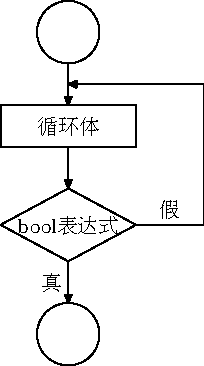
\includegraphics{graph/do-1.pdf}
    \caption{do工作流程}
  \label{fig:do_workflow}
\end{figure}

\begin{lstlisting}
#!/bin/sh

# numberlines - A simple alternative to cat -n, etc.

for filename
do
    linecount="1"
    while read line
    do
        echo "${linecount}: $line"
        linecount="$(($linecount + 1))"
    done < $filename
done
exit 0
\end{lstlisting}

\subsection{while结构}

\begin{figure}[!htbp]
  \centering
  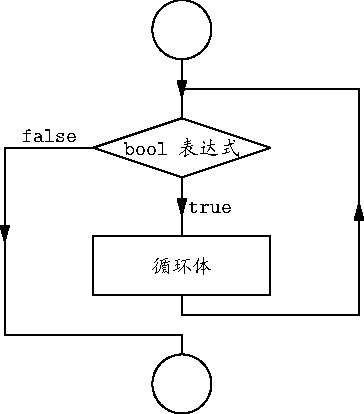
\includegraphics{graph/while.pdf}
    \caption{while工作流程}
  \label{fig:while_workflow}
\end{figure}

\lstinputlisting[aboveskip=5pt,belowskip=5pt,language=bash]{src/shell03.sh}

我们可以将while循环和专用命令“:”结合使用来定义。由于循环固有的一个特性,
当条件永远不被满足时,就会产生一个无限循环。定义一个while无限循环可以使
用如下三种命令:

\begin{enumerate}
\item true命令 \- 不做任何事情,表示成功,总是返回退出状态码0
\item false命令 \- 不做任何事情,表示失败,总是返回退出状态码1
\item :命令 \- 无作用,此命令也不做任何事情,总是返回退出状态码0
\end{enumerate}

\section{操作字符串}

\section{函数}

当我们的脚本大到一定程度时,使用函数则可以简化脚本,使程序结构更为清晰。

\section{信号捕捉}

\begin{verbatim}
trap可以捕捉信号,根据捕捉到的信号,执行响应的操作。
语法:
trap 'action' SIGNAL
\end{verbatim}

\section{开机脚本启动顺序}

\section{一个实例}

\lstinputlisting[aboveskip=5pt,belowskip=5pt,language=bash]{src/shell04.sh}

下面是该脚本的输出结果:

\begin{lstlisting}[numbers=none,aboveskip=5pt,belowskip=5pt]
System Report for richard on Tue Sep 23 21:34:22 CST 2014

Hostname: richard NIS Domain: (none)
Processor: 
Running at 4585.16
4585.16
4585.16
4585.16 bogomips with 3072 KB
3072 KB
3072 KB
3072 KB cache

OS Type: Linux Kernel:3.13.0-35-generic
Kernel Compile #62-Ubuntu on
Uptime: .08 days
Memory: 6003456 kB Free:   : 100
Swap: 6180860 kB Free:   : 100

Load Avderage:0.63 0.69 0.61 
Process Count:  total 1 running sleeping 0 stopped 0 zombie
\end{lstlisting}
